% Options for packages loaded elsewhere
\PassOptionsToPackage{unicode}{hyperref}
\PassOptionsToPackage{hyphens}{url}
\PassOptionsToPackage{dvipsnames,svgnames,x11names}{xcolor}
\documentclass[
]{article}
\usepackage{xcolor}
\usepackage[margin=1in]{geometry}
\usepackage{amsmath,amssymb}
\setcounter{secnumdepth}{-\maxdimen} % remove section numbering
\usepackage{iftex}
\ifPDFTeX
  \usepackage[T1]{fontenc}
  \usepackage[utf8]{inputenc}
  \usepackage{textcomp} % provide euro and other symbols
\else % if luatex or xetex
  \usepackage{unicode-math} % this also loads fontspec
  \defaultfontfeatures{Scale=MatchLowercase}
  \defaultfontfeatures[\rmfamily]{Ligatures=TeX,Scale=1}
\fi
\usepackage{lmodern}
\ifPDFTeX\else
  % xetex/luatex font selection
\fi
% Use upquote if available, for straight quotes in verbatim environments
\IfFileExists{upquote.sty}{\usepackage{upquote}}{}
\IfFileExists{microtype.sty}{% use microtype if available
  \usepackage[]{microtype}
  \UseMicrotypeSet[protrusion]{basicmath} % disable protrusion for tt fonts
}{}
\makeatletter
\@ifundefined{KOMAClassName}{% if non-KOMA class
  \IfFileExists{parskip.sty}{%
    \usepackage{parskip}
  }{% else
    \setlength{\parindent}{0pt}
    \setlength{\parskip}{6pt plus 2pt minus 1pt}}
}{% if KOMA class
  \KOMAoptions{parskip=half}}
\makeatother
\usepackage{color}
\usepackage{fancyvrb}
\newcommand{\VerbBar}{|}
\newcommand{\VERB}{\Verb[commandchars=\\\{\}]}
\DefineVerbatimEnvironment{Highlighting}{Verbatim}{commandchars=\\\{\}}
% Add ',fontsize=\small' for more characters per line
\usepackage{framed}
\definecolor{shadecolor}{RGB}{248,248,248}
\newenvironment{Shaded}{\begin{snugshade}}{\end{snugshade}}
\newcommand{\AlertTok}[1]{\textcolor[rgb]{0.94,0.16,0.16}{#1}}
\newcommand{\AnnotationTok}[1]{\textcolor[rgb]{0.56,0.35,0.01}{\textbf{\textit{#1}}}}
\newcommand{\AttributeTok}[1]{\textcolor[rgb]{0.13,0.29,0.53}{#1}}
\newcommand{\BaseNTok}[1]{\textcolor[rgb]{0.00,0.00,0.81}{#1}}
\newcommand{\BuiltInTok}[1]{#1}
\newcommand{\CharTok}[1]{\textcolor[rgb]{0.31,0.60,0.02}{#1}}
\newcommand{\CommentTok}[1]{\textcolor[rgb]{0.56,0.35,0.01}{\textit{#1}}}
\newcommand{\CommentVarTok}[1]{\textcolor[rgb]{0.56,0.35,0.01}{\textbf{\textit{#1}}}}
\newcommand{\ConstantTok}[1]{\textcolor[rgb]{0.56,0.35,0.01}{#1}}
\newcommand{\ControlFlowTok}[1]{\textcolor[rgb]{0.13,0.29,0.53}{\textbf{#1}}}
\newcommand{\DataTypeTok}[1]{\textcolor[rgb]{0.13,0.29,0.53}{#1}}
\newcommand{\DecValTok}[1]{\textcolor[rgb]{0.00,0.00,0.81}{#1}}
\newcommand{\DocumentationTok}[1]{\textcolor[rgb]{0.56,0.35,0.01}{\textbf{\textit{#1}}}}
\newcommand{\ErrorTok}[1]{\textcolor[rgb]{0.64,0.00,0.00}{\textbf{#1}}}
\newcommand{\ExtensionTok}[1]{#1}
\newcommand{\FloatTok}[1]{\textcolor[rgb]{0.00,0.00,0.81}{#1}}
\newcommand{\FunctionTok}[1]{\textcolor[rgb]{0.13,0.29,0.53}{\textbf{#1}}}
\newcommand{\ImportTok}[1]{#1}
\newcommand{\InformationTok}[1]{\textcolor[rgb]{0.56,0.35,0.01}{\textbf{\textit{#1}}}}
\newcommand{\KeywordTok}[1]{\textcolor[rgb]{0.13,0.29,0.53}{\textbf{#1}}}
\newcommand{\NormalTok}[1]{#1}
\newcommand{\OperatorTok}[1]{\textcolor[rgb]{0.81,0.36,0.00}{\textbf{#1}}}
\newcommand{\OtherTok}[1]{\textcolor[rgb]{0.56,0.35,0.01}{#1}}
\newcommand{\PreprocessorTok}[1]{\textcolor[rgb]{0.56,0.35,0.01}{\textit{#1}}}
\newcommand{\RegionMarkerTok}[1]{#1}
\newcommand{\SpecialCharTok}[1]{\textcolor[rgb]{0.81,0.36,0.00}{\textbf{#1}}}
\newcommand{\SpecialStringTok}[1]{\textcolor[rgb]{0.31,0.60,0.02}{#1}}
\newcommand{\StringTok}[1]{\textcolor[rgb]{0.31,0.60,0.02}{#1}}
\newcommand{\VariableTok}[1]{\textcolor[rgb]{0.00,0.00,0.00}{#1}}
\newcommand{\VerbatimStringTok}[1]{\textcolor[rgb]{0.31,0.60,0.02}{#1}}
\newcommand{\WarningTok}[1]{\textcolor[rgb]{0.56,0.35,0.01}{\textbf{\textit{#1}}}}
\usepackage{longtable,booktabs,array}
\newcounter{none} % for unnumbered tables
\usepackage{calc} % for calculating minipage widths
% Correct order of tables after \paragraph or \subparagraph
\usepackage{etoolbox}
\makeatletter
\patchcmd\longtable{\par}{\if@noskipsec\mbox{}\fi\par}{}{}
\makeatother
% Allow footnotes in longtable head/foot
\IfFileExists{footnotehyper.sty}{\usepackage{footnotehyper}}{\usepackage{footnote}}
\makesavenoteenv{longtable}
\usepackage{graphicx}
\makeatletter
\newsavebox\pandoc@box
\newcommand*\pandocbounded[1]{% scales image to fit in text height/width
  \sbox\pandoc@box{#1}%
  \Gscale@div\@tempa{\textheight}{\dimexpr\ht\pandoc@box+\dp\pandoc@box\relax}%
  \Gscale@div\@tempb{\linewidth}{\wd\pandoc@box}%
  \ifdim\@tempb\p@<\@tempa\p@\let\@tempa\@tempb\fi% select the smaller of both
  \ifdim\@tempa\p@<\p@\scalebox{\@tempa}{\usebox\pandoc@box}%
  \else\usebox{\pandoc@box}%
  \fi%
}
% Set default figure placement to htbp
\def\fps@figure{htbp}
\makeatother
\setlength{\emergencystretch}{3em} % prevent overfull lines
\providecommand{\tightlist}{%
  \setlength{\itemsep}{0pt}\setlength{\parskip}{0pt}}
\usepackage{bookmark}
\IfFileExists{xurl.sty}{\usepackage{xurl}}{} % add URL line breaks if available
\urlstyle{same}
% fallback for those not using the hyperref driver hyperxmp:
\makeatletter
\@ifundefined{xmpquote}{\newcommand{\xmpquote}[1]{#1}}{}
\makeatother
\hypersetup{
  pdftitle={Order Shipment Analysis},
  pdfauthor={Demetri Bichara},
  colorlinks=true,
  linkcolor={Maroon},
  filecolor={Maroon},
  citecolor={Blue},
  urlcolor={blue},
  pdfcreator={LaTeX via pandoc}}

\title{Order Shipment Analysis}
\author{Demetri Bichara}
\date{2026-11-07}

\begin{document}
\maketitle

{
\setcounter{tocdepth}{2}
\tableofcontents
}
\section{Part 1 - Goal A:}\label{part-1---goal-a}

Provide the following information for any instance:

\begin{enumerate}
\def\labelenumi{\arabic{enumi}.}
\tightlist
\item
  \textbf{Order \#}
\item
  \textbf{Item Name}
\item
  \textbf{Quantity}
\item
  \textbf{Total value} (price x quantity)
\end{enumerate}

\subsection{Solution}\label{p1ASolution}

\begin{Shaded}
\begin{Highlighting}[]
\NormalTok{unshipped }\OtherTok{\textless{}{-}}\NormalTok{ orders }\SpecialCharTok{|\textgreater{}}
  \FunctionTok{left\_join}\NormalTok{(shipments, }\AttributeTok{by =} \StringTok{\textquotesingle{}id\textquotesingle{}}\NormalTok{, }\AttributeTok{relationship =} \StringTok{\textquotesingle{}one{-}to{-}one\textquotesingle{}}\NormalTok{) }\SpecialCharTok{|\textgreater{}}
  \FunctionTok{left\_join}\NormalTok{(items, }\AttributeTok{by =} \StringTok{\textquotesingle{}item\_id\textquotesingle{}}\NormalTok{, }\AttributeTok{relationship =} \StringTok{\textquotesingle{}many{-}to{-}one\textquotesingle{}}\NormalTok{) }\SpecialCharTok{|\textgreater{}}
  \FunctionTok{mutate}\NormalTok{(}
    \AttributeTok{why\_unshipped =} \FunctionTok{case\_when}\NormalTok{(}
      \FunctionTok{is.na}\NormalTok{(status) }\SpecialCharTok{\textasciitilde{}} \StringTok{"No shipment record"}\NormalTok{, }
\NormalTok{      status }\SpecialCharTok{==} \StringTok{"Pending"} \SpecialCharTok{\textasciitilde{}} \StringTok{"Not yet shipped"}\NormalTok{,}
      \ConstantTok{TRUE} \SpecialCharTok{\textasciitilde{}} \ConstantTok{NA}\NormalTok{), }
    \AttributeTok{total\_value =}\NormalTok{ price }\SpecialCharTok{*}\NormalTok{ quantity) }\SpecialCharTok{|\textgreater{}} 
  \FunctionTok{filter}\NormalTok{(}\SpecialCharTok{!}\FunctionTok{is.na}\NormalTok{(why\_unshipped)) }\SpecialCharTok{|\textgreater{}}
  \FunctionTok{select}\NormalTok{(order\_id, id, name, quantity, total\_value, why\_unshipped) }\SpecialCharTok{|\textgreater{}} 
  \FunctionTok{arrange}\NormalTok{(order\_id, id) }
\end{Highlighting}
\end{Shaded}

\begin{Shaded}
\begin{Highlighting}[]
\NormalTok{unshipped}
\end{Highlighting}
\end{Shaded}

{\def\LTcaptype{none} % do not increment counter
\begin{longtable}[]{@{}
  >{\raggedleft\arraybackslash}p{(\linewidth - 10\tabcolsep) * \real{0.1139}}
  >{\raggedleft\arraybackslash}p{(\linewidth - 10\tabcolsep) * \real{0.0633}}
  >{\raggedright\arraybackslash}p{(\linewidth - 10\tabcolsep) * \real{0.3165}}
  >{\raggedleft\arraybackslash}p{(\linewidth - 10\tabcolsep) * \real{0.1139}}
  >{\raggedleft\arraybackslash}p{(\linewidth - 10\tabcolsep) * \real{0.1519}}
  >{\raggedright\arraybackslash}p{(\linewidth - 10\tabcolsep) * \real{0.2405}}@{}}
\toprule\noalign{}
\begin{minipage}[b]{\linewidth}\raggedleft
order\_id
\end{minipage} & \begin{minipage}[b]{\linewidth}\raggedleft
id
\end{minipage} & \begin{minipage}[b]{\linewidth}\raggedright
name
\end{minipage} & \begin{minipage}[b]{\linewidth}\raggedleft
quantity
\end{minipage} & \begin{minipage}[b]{\linewidth}\raggedleft
total\_value
\end{minipage} & \begin{minipage}[b]{\linewidth}\raggedright
why\_unshipped
\end{minipage} \\
\midrule\noalign{}
\endhead
\bottomrule\noalign{}
\endlastfoot
65 & 275 & Network Attached Storage & 20 & 8000 & No shipment record \\
70 & 292 & Monitor 27-inch & 8 & 2240 & No shipment record \\
70 & 294 & External SSD 1TB & 2 & 240 & No shipment record \\
70 & 297 & Extended Warranty 3yr & 5 & 1000 & No shipment record \\
120 & 541 & DisplayPort Cable & 34 & 476 & No shipment record \\
125 & 570 & Motherboard - Micro ATX & 1 & 150 & No shipment record \\
140 & 637 & Wireless Keyboard & 33 & 1485 & No shipment record \\
162 & 750 & GPU - Mid Range & 25 & 13750 & No shipment record \\
166 & 765 & Network Attached Storage & 5 & 2000 & No shipment record \\
186 & 860 & Wi-Fi USB Adapter & 14 & 350 & No shipment record \\
297 & 1352 & Motherboard - Mini ITX & 17 & 3060 & No shipment record \\
300 & 1367 & RAM - 8GB & 20 & 3000 & No shipment record \\
319 & 1451 & PC Case - Mid Tower & 24 & 2160 & No shipment record \\
322 & 1462 & Mini PC & 31 & 13950 & No shipment record \\
333 & 1499 & Wireless Mouse & 17 & 510 & No shipment record \\
337 & 1526 & Chromebook & 11 & 3850 & No shipment record \\
374 & 1680 & Laptop Stand & 9 & 315 & No shipment record \\
411 & 1812 & Gaming Mouse & 16 & 960 & No shipment record \\
444 & 1960 & PC Case - Full Tower & 19 & 3040 & No shipment record \\
483 & 2137 & Bluetooth Speaker & 28 & 2520 & Not yet shipped \\
483 & 2138 & RAM - 32GB & 17 & 9350 & Not yet shipped \\
483 & 2139 & Case Fan 120mm & 17 & 204 & Not yet shipped \\
483 & 2140 & USB-C Cable 1m & 4 & 40 & Not yet shipped \\
483 & 2142 & Motherboard - Mini ITX & 26 & 4680 & Not yet shipped \\
484 & 2144 & SD Card 128GB & 13 & 260 & Not yet shipped \\
484 & 2145 & Smartphone & 9 & 7200 & Not yet shipped \\
484 & 2146 & SSD 500GB & 3 & 210 & Not yet shipped \\
484 & 2147 & Monitor Arm & 27 & 2025 & Not yet shipped \\
484 & 2148 & Power Supply 1000W & 32 & 5760 & Not yet shipped \\
487 & 2152 & SD Card 128GB & 2 & 40 & Not yet shipped \\
487 & 2153 & Laptop Bag & 24 & 1320 & Not yet shipped \\
487 & 2154 & Surge Protector & 6 & 150 & Not yet shipped \\
487 & 2155 & Motherboard - Mini ITX & 19 & 3420 & Not yet shipped \\
487 & 2156 & USB Flash Drive 64GB & 4 & 48 & No shipment record \\
487 & 2157 & HDD 8TB & 29 & 4640 & Not yet shipped \\
487 & 2158 & CPU - Mid Range & 22 & 7040 & Not yet shipped \\
487 & 2159 & USB-C Cable 1m & 28 & 280 & Not yet shipped \\
488 & 2161 & GPU - Mid Range & 32 & 17600 & Not yet shipped \\
491 & 2168 & Ethernet Cable 10m & 30 & 450 & Not yet shipped \\
491 & 2169 & Operating System License & 22 & 3080 & Not yet shipped \\
491 & 2170 & Motherboard - ATX & 22 & 4840 & Not yet shipped \\
491 & 2171 & RAM - 32GB & 35 & 19250 & Not yet shipped \\
491 & 2172 & Flatbed Scanner & 13 & 1820 & Not yet shipped \\
491 & 2173 & GPU - Entry Level & 25 & 7000 & Not yet shipped \\
491 & 2174 & Power Bank 20000mAh & 14 & 630 & Not yet shipped \\
494 & 2188 & Ethernet Cable 2m & 7 & 42 & Not yet shipped \\
494 & 2189 & Motherboard - Micro ATX & 20 & 3000 & Not yet shipped \\
495 & 2190 & SD Card 128GB & 14 & 280 & Not yet shipped \\
495 & 2191 & HDD 8TB & 30 & 4800 & Not yet shipped \\
495 & 2192 & GPU - Mid Range & 25 & 13750 & Not yet shipped \\
495 & 2193 & Monitor 32-inch 4K & 26 & 12480 & Not yet shipped \\
495 & 2194 & Wireless Keyboard & 18 & 810 & Not yet shipped \\
495 & 2195 & Ethernet Cable 2m & 12 & 72 & Not yet shipped \\
496 & 2197 & Tablet 12-inch & 26 & 19500 & Not yet shipped \\
496 & 2199 & Ergonomic Mouse & 10 & 700 & Not yet shipped \\
497 & 2202 & Wireless Keyboard & 16 & 720 & Not yet shipped \\
497 & 2203 & HDD 8TB & 20 & 3200 & Not yet shipped \\
497 & 2204 & HDMI Cable 2m & 2 & 18 & Not yet shipped \\
498 & 2205 & RAM - 32GB & 11 & 6050 & Not yet shipped \\
498 & 2206 & Wireless Access Point & 3 & 420 & Not yet shipped \\
498 & 2207 & Monitor 27-inch & 11 & 3080 & Not yet shipped \\
498 & 2208 & SSD 4TB & 31 & 11160 & Not yet shipped \\
498 & 2209 & All-in-One PC & 24 & 30000 & Not yet shipped \\
498 & 2210 & RAM - 16GB & 10 & 3000 & Not yet shipped \\
498 & 2211 & Laptop Stand & 20 & 700 & Not yet shipped \\
498 & 2212 & USB-C Cable 1m & 33 & 330 & Not yet shipped \\
499 & 2213 & SD Card 128GB & 30 & 600 & Not yet shipped \\
499 & 2214 & External HDD 4TB & 10 & 1050 & Not yet shipped \\
499 & 2215 & Chromebook & 24 & 8400 & Not yet shipped \\
500 & 2216 & GPU - Mid Range & 20 & 11000 & Not yet shipped \\
500 & 2217 & Laptop Bag & 18 & 990 & Not yet shipped \\
\end{longtable}
}

\begin{Shaded}
\begin{Highlighting}[]
\NormalTok{unshipped }\SpecialCharTok{|\textgreater{}}
  \FunctionTok{summarize}\NormalTok{(}
    \AttributeTok{missing\_prices =} \FunctionTok{sum}\NormalTok{(}\FunctionTok{is.na}\NormalTok{(total\_value))}
\NormalTok{    )}
\end{Highlighting}
\end{Shaded}

{\def\LTcaptype{none} % do not increment counter
\begin{longtable}[]{@{}r@{}}
\toprule\noalign{}
missing\_prices \\
\midrule\noalign{}
\endhead
\bottomrule\noalign{}
\endlastfoot
0 \\
\end{longtable}
}

\begin{Shaded}
\begin{Highlighting}[]
\NormalTok{unshipped }\SpecialCharTok{|\textgreater{}}
  \FunctionTok{summarize}\NormalTok{(}
    \AttributeTok{affected\_orders =} \FunctionTok{n\_distinct}\NormalTok{(order\_id),}
    \AttributeTok{unshipped\_lines =} \FunctionTok{n}\NormalTok{(),}
    \AttributeTok{total\_unshipped\_value =} \FunctionTok{sum}\NormalTok{(total\_value)}
\NormalTok{  )}
\end{Highlighting}
\end{Shaded}

{\def\LTcaptype{none} % do not increment counter
\begin{longtable}[]{@{}rrr@{}}
\toprule\noalign{}
affected\_orders & unshipped\_lines & total\_unshipped\_value \\
\midrule\noalign{}
\endhead
\bottomrule\noalign{}
\endlastfoot
29 & 71 & 300545 \\
\end{longtable}
}

\begin{Shaded}
\begin{Highlighting}[]
\NormalTok{unshipped }\SpecialCharTok{|\textgreater{}}
  \FunctionTok{group\_by}\NormalTok{(why\_unshipped) }\SpecialCharTok{|\textgreater{}}
  \FunctionTok{summarize}\NormalTok{(}
    \AttributeTok{affected\_orders =} \FunctionTok{n\_distinct}\NormalTok{(order\_id),}
    \AttributeTok{unshipped\_lines =} \FunctionTok{n}\NormalTok{(),}
    \AttributeTok{total\_unshipped\_value =} \FunctionTok{sum}\NormalTok{(total\_value),}
    \AttributeTok{.groups =} \StringTok{"drop"}
\NormalTok{  )}
\end{Highlighting}
\end{Shaded}

{\def\LTcaptype{none} % do not increment counter
\begin{longtable}[]{@{}
  >{\raggedright\arraybackslash}p{(\linewidth - 6\tabcolsep) * \real{0.2603}}
  >{\raggedleft\arraybackslash}p{(\linewidth - 6\tabcolsep) * \real{0.2192}}
  >{\raggedleft\arraybackslash}p{(\linewidth - 6\tabcolsep) * \real{0.2192}}
  >{\raggedleft\arraybackslash}p{(\linewidth - 6\tabcolsep) * \real{0.3014}}@{}}
\toprule\noalign{}
\begin{minipage}[b]{\linewidth}\raggedright
why\_unshipped
\end{minipage} & \begin{minipage}[b]{\linewidth}\raggedleft
affected\_orders
\end{minipage} & \begin{minipage}[b]{\linewidth}\raggedleft
unshipped\_lines
\end{minipage} & \begin{minipage}[b]{\linewidth}\raggedleft
total\_unshipped\_value
\end{minipage} \\
\midrule\noalign{}
\endhead
\bottomrule\noalign{}
\endlastfoot
No shipment record & 18 & 20 & 60584 \\
Not yet shipped & 12 & 51 & 239961 \\
\end{longtable}
}

To ID unshipped order lines, I first established the relationships
between the orders, shipments, and items tables. The id column was found
to be the most probable order-line identifier shared between orders and
shipments. I ID'd 20 order lines that did not have a corresponding
shipment record, and 51 shipment statuses that are Pending. A Complete
shipment is assumed to fulfill the entire ordered quantity, since
shipments don't specify shipment-level quantities. Lastly, I calculated
total unshipped value for each unshipped order line via price *
quantity.

\subsection{Methodology}\label{method}

First, we need to know how to map 1 order to their corresponding
shipments. The most probable path is a left joining of the shipments CSV
on the orders CSV, which preserves every order line item (including the
order line items without corresponding shipments).

From inspecting the data in the two CSV's with RStudio, I can see the
orders.id column has the same range as the shipments.id column. Due to
this similarity, I think that the best way to left join the two tables
is by using the \texttt{id} column for equality checking. If correct,
the relationship for the two \texttt{id} columns is 1:0-1 (0 in the case
of a missed shipment).

We can do the same duplicate-checking test to start to assert the
truthfulness of the described many-to-one relationship for the
\texttt{item\_id} column across the two tables orders and items.

Checking for any duplicate values in the \texttt{id} column within both
tables, which would break the proposed 1:0-1 mapping.

\subsubsection{1:0-1 test-A:}\label{test-a}

\begin{Shaded}
\begin{Highlighting}[]
\FunctionTok{any}\NormalTok{(}\FunctionTok{duplicated}\NormalTok{(shipments}\SpecialCharTok{$}\NormalTok{id)) }\CommentTok{\# should be FALSE}
\end{Highlighting}
\end{Shaded}

\begin{verbatim}
## [1] FALSE
\end{verbatim}

\begin{Shaded}
\begin{Highlighting}[]
\FunctionTok{any}\NormalTok{(}\FunctionTok{duplicated}\NormalTok{(orders}\SpecialCharTok{$}\NormalTok{id)) }\CommentTok{\# should be FALSE }
\end{Highlighting}
\end{Shaded}

\begin{verbatim}
## [1] FALSE
\end{verbatim}

\subsubsection{N:1 test-A:}\label{n1-test-a}

\begin{Shaded}
\begin{Highlighting}[]
\FunctionTok{any}\NormalTok{(}\FunctionTok{duplicated}\NormalTok{(orders}\SpecialCharTok{$}\NormalTok{item\_id)) }\CommentTok{\# should be TRUE (many{-}to{-}one)}
\end{Highlighting}
\end{Shaded}

\begin{verbatim}
## [1] TRUE
\end{verbatim}

\begin{Shaded}
\begin{Highlighting}[]
\FunctionTok{any}\NormalTok{(}\FunctionTok{duplicated}\NormalTok{(items}\SpecialCharTok{$}\NormalTok{item\_id)) }\CommentTok{\# should be FALSE}
\end{Highlighting}
\end{Shaded}

\begin{verbatim}
## [1] FALSE
\end{verbatim}

Since there aren't duplicates in the \texttt{id} column of either the
shipments CSV or the orders CSV, we can further test my proposed
relationship between the two tables by checking whether all \texttt{id}
values in the shipment CSV exist in the \texttt{id} column of the orders
CSV with an anti join. This will not fail on missed shipments since
anti\_join(shipments, orders) only tests whether shipment records have
corresponding order lines. We can do the same check with the
\texttt{item\_id} column across the tables orders and items.

\subsubsection{1:0-1 test-B:}\label{test-b}

\begin{Shaded}
\begin{Highlighting}[]
\NormalTok{shipments }\SpecialCharTok{|\textgreater{}} \FunctionTok{anti\_join}\NormalTok{(orders, }\AttributeTok{by =} \StringTok{\textquotesingle{}id\textquotesingle{}}\NormalTok{) }
\end{Highlighting}
\end{Shaded}

{\def\LTcaptype{none} % do not increment counter
\begin{longtable}[]{@{}rrll@{}}
\toprule\noalign{}
shipment\_id & id & status & ship\_date \\
\midrule\noalign{}
\endhead
\bottomrule\noalign{}
\endlastfoot
\end{longtable}
}

0 rows missing a corresponding id!

\subsubsection{N:1 test-B:}\label{n1-test-b}

\begin{Shaded}
\begin{Highlighting}[]
\NormalTok{orders }\SpecialCharTok{|\textgreater{}} \FunctionTok{anti\_join}\NormalTok{(items, }\AttributeTok{by =} \StringTok{\textquotesingle{}item\_id\textquotesingle{}}\NormalTok{)}
\end{Highlighting}
\end{Shaded}

{\def\LTcaptype{none} % do not increment counter
\begin{longtable}[]{@{}rrlrlr@{}}
\toprule\noalign{}
id & order\_id & order\_date & item\_id & company & quantity \\
\midrule\noalign{}
\endhead
\bottomrule\noalign{}
\endlastfoot
\end{longtable}
}

0 rows missing a corresponding id!

Since all testing passed so far, we can further test the understood
relationships by setting an expected relationship during the joining
process.

\begin{Shaded}
\begin{Highlighting}[]
\NormalTok{orders }\SpecialCharTok{|\textgreater{}} 
  \FunctionTok{left\_join}\NormalTok{(shipments, }\AttributeTok{by =} \StringTok{\textquotesingle{}id\textquotesingle{}}\NormalTok{, }\AttributeTok{relationship =} \StringTok{\textquotesingle{}one{-}to{-}one\textquotesingle{}}\NormalTok{) }\SpecialCharTok{|\textgreater{}}
  \FunctionTok{left\_join}\NormalTok{(items, }\AttributeTok{by =} \StringTok{\textquotesingle{}item\_id\textquotesingle{}}\NormalTok{, }\AttributeTok{relationship =} \StringTok{\textquotesingle{}many{-}to{-}one\textquotesingle{}}\NormalTok{)}
\end{Highlighting}
\end{Shaded}

The joins executed without error, meaning matches during the join did
not violate the declared relationships (wouldn't catch a missing
shipment, okay because the cardinality is 1:0-1). The checks
collectively provide strong evidence to move forward with the
understanding.

Now that we are confident in the relationships, we can start to
investigate missing shipments by reversing the anti-join direction from
`1:0-1 test-B'. This would show all order line items that did not have a
corresponding shipment. Importantly, this would not catch all unshipped
order lines by itself, since the corresponding status might not be
`Complete'. Moreover, since the shipments table doesn't contain a
quantity column, we will assume that a shipment line entry / row with
the `Complete' status indicates the entire corresponding quantity was
sent.

\begin{Shaded}
\begin{Highlighting}[]
\NormalTok{orders }\SpecialCharTok{|\textgreater{}} \FunctionTok{anti\_join}\NormalTok{(shipments, }\AttributeTok{by =} \StringTok{\textquotesingle{}id\textquotesingle{}}\NormalTok{)}
\end{Highlighting}
\end{Shaded}

{\def\LTcaptype{none} % do not increment counter
\begin{longtable}[]{@{}rrlrlr@{}}
\toprule\noalign{}
id & order\_id & order\_date & item\_id & company & quantity \\
\midrule\noalign{}
\endhead
\bottomrule\noalign{}
\endlastfoot
275 & 65 & 2025-12-16 & 73 & Qualcomm & 20 \\
292 & 70 & 2025-12-17 & 47 & Starbucks & 8 \\
294 & 70 & 2025-12-17 & 24 & Starbucks & 2 \\
297 & 70 & 2025-12-17 & 98 & Starbucks & 5 \\
541 & 120 & 2026-01-26 & 79 & Intel & 34 \\
570 & 125 & 2026-01-30 & 35 & Microsoft & 1 \\
637 & 140 & 2026-02-09 & 52 & Apple & 33 \\
750 & 162 & 2026-02-23 & 32 & Delta Air Lines & 25 \\
765 & 166 & 2026-02-25 & 73 & Qualcomm & 5 \\
860 & 186 & 2026-03-14 & 71 & FedEx & 14 \\
1352 & 297 & 2026-06-04 & 36 & Dell Technologies & 17 \\
1367 & 300 & 2026-06-07 & 14 & Humana & 20 \\
1451 & 319 & 2026-06-19 & 40 & Berkshire Hathaway & 24 \\
1462 & 322 & 2026-06-20 & 8 & IBM & 31 \\
1499 & 333 & 2026-06-30 & 54 & UPS & 17 \\
1526 & 337 & 2026-07-01 & 6 & Home Depot & 11 \\
1680 & 374 & 2026-08-11 & 84 & Honeywell & 9 \\
1812 & 411 & 2026-09-05 & 55 & Adobe & 16 \\
1960 & 444 & 2026-09-29 & 41 & Walmart & 19 \\
2156 & 487 & 2026-10-25 & 26 & Amazon & 4 \\
\end{longtable}
}

Checks for orders without matching shipment records: matched 20 order
line items

\begin{Shaded}
\begin{Highlighting}[]
\FunctionTok{unique}\NormalTok{(shipments}\SpecialCharTok{$}\NormalTok{status) }
\end{Highlighting}
\end{Shaded}

\begin{verbatim}
## [1] "Complete" "Pending"
\end{verbatim}

2 possible values for a status entry \{`Complete', `Pending'\} (no na).
The literal meaning of \texttt{Pending} might be loose: if its been
pending for 9 months, is that an anomaly or a true shipping time? The
most recent date in the shipments table's \texttt{ship\_date} column is
11-02 of this year (2026), so we can use that point for detecting zombie
shipments with an aging threshold. However, for purposes of this beta,
we can further analysis knowing only
`pending'\textless-\textgreater{}`not yet shipped'.

As to verify the data quality before further analysis, we can also make
sure no shipment dates precede their order dates.

\begin{Shaded}
\begin{Highlighting}[]
\NormalTok{orders }\SpecialCharTok{|\textgreater{}}
  \FunctionTok{left\_join}\NormalTok{(shipments, }\AttributeTok{by =} \StringTok{\textquotesingle{}id\textquotesingle{}}\NormalTok{) }\SpecialCharTok{|\textgreater{}}
  \FunctionTok{filter}\NormalTok{(}\SpecialCharTok{!}\FunctionTok{is.na}\NormalTok{(ship\_date), ship\_date }\SpecialCharTok{\textless{}}\NormalTok{ order\_date)}
\end{Highlighting}
\end{Shaded}

{\def\LTcaptype{none} % do not increment counter
\begin{longtable}[]{@{}
  >{\raggedleft\arraybackslash}p{(\linewidth - 16\tabcolsep) * \real{0.0390}}
  >{\raggedleft\arraybackslash}p{(\linewidth - 16\tabcolsep) * \real{0.1169}}
  >{\raggedright\arraybackslash}p{(\linewidth - 16\tabcolsep) * \real{0.1429}}
  >{\raggedleft\arraybackslash}p{(\linewidth - 16\tabcolsep) * \real{0.1039}}
  >{\raggedright\arraybackslash}p{(\linewidth - 16\tabcolsep) * \real{0.1039}}
  >{\raggedleft\arraybackslash}p{(\linewidth - 16\tabcolsep) * \real{0.1169}}
  >{\raggedleft\arraybackslash}p{(\linewidth - 16\tabcolsep) * \real{0.1558}}
  >{\raggedright\arraybackslash}p{(\linewidth - 16\tabcolsep) * \real{0.0909}}
  >{\raggedright\arraybackslash}p{(\linewidth - 16\tabcolsep) * \real{0.1299}}@{}}
\toprule\noalign{}
\begin{minipage}[b]{\linewidth}\raggedleft
id
\end{minipage} & \begin{minipage}[b]{\linewidth}\raggedleft
order\_id
\end{minipage} & \begin{minipage}[b]{\linewidth}\raggedright
order\_date
\end{minipage} & \begin{minipage}[b]{\linewidth}\raggedleft
item\_id
\end{minipage} & \begin{minipage}[b]{\linewidth}\raggedright
company
\end{minipage} & \begin{minipage}[b]{\linewidth}\raggedleft
quantity
\end{minipage} & \begin{minipage}[b]{\linewidth}\raggedleft
shipment\_id
\end{minipage} & \begin{minipage}[b]{\linewidth}\raggedright
status
\end{minipage} & \begin{minipage}[b]{\linewidth}\raggedright
ship\_date
\end{minipage} \\
\midrule\noalign{}
\endhead
\bottomrule\noalign{}
\endlastfoot
\end{longtable}
}

Matches 0 orders who have an earlier corresponding shipment record.

Same type on the two \texttt{*\_date} fields makes the comparison
possible, so we should test that:

\begin{Shaded}
\begin{Highlighting}[]
\FunctionTok{class}\NormalTok{(orders}\SpecialCharTok{$}\NormalTok{order\_date)}
\end{Highlighting}
\end{Shaded}

\begin{verbatim}
## [1] "Date"
\end{verbatim}

\begin{Shaded}
\begin{Highlighting}[]
\FunctionTok{class}\NormalTok{(shipments}\SpecialCharTok{$}\NormalTok{ship\_date)}
\end{Highlighting}
\end{Shaded}

\begin{verbatim}
## [1] "Date"
\end{verbatim}

While \{``Complete'', ``Pending''\} are the only two values in the
\texttt{status} column, it's worth it to check for shipments marked as
\texttt{Complete} without it's corresponding evidence (the ship date).
While a missing ship date doesn't automatically mean a false status
entry, we do not have access to the underlying business logic generating
the DB, so we can mark the results from all shipments who have a status
= `Complete' and no ship date.

\begin{Shaded}
\begin{Highlighting}[]
\NormalTok{shipments }\SpecialCharTok{|\textgreater{}}
  \FunctionTok{filter}\NormalTok{(}
\NormalTok{    (status }\SpecialCharTok{==} \StringTok{"Complete"} \SpecialCharTok{\&} \FunctionTok{is.na}\NormalTok{(ship\_date)) }\SpecialCharTok{|}
\NormalTok{      (status }\SpecialCharTok{==} \StringTok{"Pending"} \SpecialCharTok{\&} \SpecialCharTok{!}\FunctionTok{is.na}\NormalTok{(ship\_date)) }\CommentTok{\# check the reverse also to make}
    \CommentTok{\#                                             sure business logic }
    \CommentTok{\#                                              understanding is right}
    \CommentTok{\#                                 (pending shipments cannot have dates)}
\NormalTok{  ) }
\end{Highlighting}
\end{Shaded}

{\def\LTcaptype{none} % do not increment counter
\begin{longtable}[]{@{}rrll@{}}
\toprule\noalign{}
shipment\_id & id & status & ship\_date \\
\midrule\noalign{}
\endhead
\bottomrule\noalign{}
\endlastfoot
\end{longtable}
}

No such case! Moreover, we have to handle any missing shipment\_id rows
as to handle `Pending' for ghost shipments

\begin{Shaded}
\begin{Highlighting}[]
\NormalTok{shipments }\SpecialCharTok{|\textgreater{}} 
  \FunctionTok{filter}\NormalTok{(}\FunctionTok{is.na}\NormalTok{(shipment\_id)) }\SpecialCharTok{|\textgreater{}}
  \FunctionTok{count}\NormalTok{(status)}
\end{Highlighting}
\end{Shaded}

{\def\LTcaptype{none} % do not increment counter
\begin{longtable}[]{@{}lr@{}}
\toprule\noalign{}
status & n \\
\midrule\noalign{}
\endhead
\bottomrule\noalign{}
\endlastfoot
Pending & 51 \\
\end{longtable}
}

Matched 51 shipment record whose status is pending without a shipment ID
(they shouldn't have it). Didn't catch any Complete order line items
without a shipment ID.

Assert we found all pending records.

\begin{Shaded}
\begin{Highlighting}[]
\NormalTok{shipments }\SpecialCharTok{|\textgreater{}}
  \FunctionTok{filter}\NormalTok{(status }\SpecialCharTok{==} \StringTok{"Pending"}\NormalTok{) }\SpecialCharTok{|\textgreater{}}
  \FunctionTok{summarize}\NormalTok{(}\AttributeTok{n =} \FunctionTok{n}\NormalTok{())}
\end{Highlighting}
\end{Shaded}

{\def\LTcaptype{none} % do not increment counter
\begin{longtable}[]{@{}r@{}}
\toprule\noalign{}
n \\
\midrule\noalign{}
\endhead
\bottomrule\noalign{}
\endlastfoot
51 \\
\end{longtable}
}

Since both tests display 51 records, we are more confident in the
understanding of the business logic.

With a strong validation / understanding of the data via the first
phase, we can now finally get the raw unshipped order line item numbers
and handle the observed cases!

\section{Part 1 - Goal B:}\label{part-1---goal-b}

Describe how you would implement a process using to alert you of
instances when orders didn't ship completely. How would you track it?
How would you automate it?

\subsection{Response}\label{p1BSolution}

\textbf{Objective}

I'd make a daily or bi-daily monitoring process that keeps track of
marked order line items and their order\_ids, and configure the
appropriate teams messaging to automatically receive notices for when an
order exceeds an agreed shipping timeframe.

\textbf{1. Detect incomplete orders}

The process would refresh the orders, shipments, and items datasets
daily. Using the relationships established in Part 1, it would join the
tables and classify each order line as Complete, Pending, or Missing
Shipment Record. If the refresh fails, I'd notify the software
maintainer.

An order would be considered fully shipped only when all its
corresponding order lines have a Complete status.

\textbf{2. Track outstanding shipments}

I would program the script to maintain a persistent table (periodically
saving/overwriting backups to disk in case of a run-time crash)
containing the order ID, order-line ID, customer, item, quantity,
unshipped value, order date, current shipment status, and why the
shipment was incomplete for each marked unshipped shipment line item.

I would include more fields for recording when the exception was first
detected, how long it has been since, whether an alert has been sent,
and if / when it's been resolved. We can remove records from the
tracking DB when the issue has been resolved for more than 30 days. We
can also use the described fields to know when to re-notify a team of
the issue.

Missing shipment records allude to incomplete order lines, so an order
should only be classified as fully shipped when every associated order
line has a Complete shipment status.

\begin{Shaded}
\begin{Highlighting}[]
\NormalTok{order\_completion }\OtherTok{\textless{}{-}}\NormalTok{ orders }\SpecialCharTok{|\textgreater{}}
  \FunctionTok{left\_join}\NormalTok{(}
\NormalTok{    shipments,}
    \AttributeTok{by =} \StringTok{"id"}\NormalTok{,}
    \AttributeTok{relationship =} \StringTok{"one{-}to{-}one"}
\NormalTok{  ) }\SpecialCharTok{|\textgreater{}}
  \FunctionTok{group\_by}\NormalTok{(order\_id) }\SpecialCharTok{|\textgreater{}}
  \FunctionTok{summarize}\NormalTok{(}
    \AttributeTok{total\_lines =} \FunctionTok{n}\NormalTok{(),}
    \AttributeTok{incomplete\_lines =} \FunctionTok{sum}\NormalTok{(}
      \FunctionTok{is.na}\NormalTok{(status) }\SpecialCharTok{|}\NormalTok{ status }\SpecialCharTok{!=} \StringTok{"Complete"}
\NormalTok{    ),}
    \AttributeTok{fully\_shipped =}\NormalTok{ incomplete\_lines }\SpecialCharTok{==} \DecValTok{0}\NormalTok{,}
    \AttributeTok{.groups =} \StringTok{"drop"}
\NormalTok{  )}

\NormalTok{order\_completion }\SpecialCharTok{|\textgreater{}}
  \FunctionTok{filter}\NormalTok{(}\SpecialCharTok{!}\NormalTok{fully\_shipped)}
\end{Highlighting}
\end{Shaded}

{\def\LTcaptype{none} % do not increment counter
\begin{longtable}[]{@{}rrrl@{}}
\toprule\noalign{}
order\_id & total\_lines & incomplete\_lines & fully\_shipped \\
\midrule\noalign{}
\endhead
\bottomrule\noalign{}
\endlastfoot
65 & 6 & 1 & FALSE \\
70 & 8 & 3 & FALSE \\
120 & 6 & 1 & FALSE \\
125 & 8 & 1 & FALSE \\
140 & 4 & 1 & FALSE \\
162 & 7 & 1 & FALSE \\
166 & 8 & 1 & FALSE \\
186 & 7 & 1 & FALSE \\
297 & 2 & 1 & FALSE \\
300 & 7 & 1 & FALSE \\
319 & 4 & 1 & FALSE \\
322 & 3 & 1 & FALSE \\
333 & 7 & 1 & FALSE \\
337 & 8 & 1 & FALSE \\
374 & 1 & 1 & FALSE \\
411 & 5 & 1 & FALSE \\
444 & 5 & 1 & FALSE \\
483 & 7 & 5 & FALSE \\
484 & 5 & 5 & FALSE \\
487 & 8 & 8 & FALSE \\
488 & 2 & 1 & FALSE \\
491 & 7 & 7 & FALSE \\
494 & 2 & 2 & FALSE \\
495 & 6 & 6 & FALSE \\
496 & 6 & 2 & FALSE \\
497 & 3 & 3 & FALSE \\
498 & 8 & 8 & FALSE \\
499 & 3 & 3 & FALSE \\
500 & 2 & 2 & FALSE \\
\end{longtable}
}

\begin{Shaded}
\begin{Highlighting}[]
\NormalTok{joined }\OtherTok{\textless{}{-}}\NormalTok{ orders }\SpecialCharTok{|\textgreater{}}
  \FunctionTok{left\_join}\NormalTok{(}
\NormalTok{    shipments,}
    \AttributeTok{by =} \StringTok{"id"}\NormalTok{,}
    \AttributeTok{relationship =} \StringTok{"one{-}to{-}one"}
\NormalTok{  )}

\NormalTok{joined }\SpecialCharTok{|\textgreater{}}
  \FunctionTok{mutate}\NormalTok{(}
    \AttributeTok{incomplete =} \FunctionTok{is.na}\NormalTok{(status) }\SpecialCharTok{|}\NormalTok{ status }\SpecialCharTok{!=} \StringTok{"Complete"}
\NormalTok{  ) }\SpecialCharTok{|\textgreater{}}
  \FunctionTok{summarize}\NormalTok{(}
    \AttributeTok{total\_lines =} \FunctionTok{n}\NormalTok{(),}
    \AttributeTok{incomplete\_lines =} \FunctionTok{sum}\NormalTok{(incomplete),}
    \AttributeTok{affected\_orders =} \FunctionTok{n\_distinct}\NormalTok{(order\_id[incomplete])}
\NormalTok{  )}
\end{Highlighting}
\end{Shaded}

{\def\LTcaptype{none} % do not increment counter
\begin{longtable}[]{@{}rrr@{}}
\toprule\noalign{}
total\_lines & incomplete\_lines & affected\_orders \\
\midrule\noalign{}
\endhead
\bottomrule\noalign{}
\endlastfoot
2217 & 71 & 29 \\
\end{longtable}
}

\begin{Shaded}
\begin{Highlighting}[]
\NormalTok{joined }\SpecialCharTok{|\textgreater{}}
  \FunctionTok{count}\NormalTok{(status)}
\end{Highlighting}
\end{Shaded}

{\def\LTcaptype{none} % do not increment counter
\begin{longtable}[]{@{}lr@{}}
\toprule\noalign{}
status & n \\
\midrule\noalign{}
\endhead
\bottomrule\noalign{}
\endlastfoot
Complete & 2146 \\
Pending & 51 \\
NA & 20 \\
\end{longtable}
}

\begin{Shaded}
\begin{Highlighting}[]
\NormalTok{order\_completion }\SpecialCharTok{|\textgreater{}}
  \FunctionTok{filter}\NormalTok{(}\SpecialCharTok{!}\NormalTok{fully\_shipped) }\SpecialCharTok{|\textgreater{}}
  \FunctionTok{summarize}\NormalTok{(}
    \AttributeTok{affected\_orders =} \FunctionTok{n\_distinct}\NormalTok{(order\_id)}
\NormalTok{  )}
\end{Highlighting}
\end{Shaded}

{\def\LTcaptype{none} % do not increment counter
\begin{longtable}[]{@{}r@{}}
\toprule\noalign{}
affected\_orders \\
\midrule\noalign{}
\endhead
\bottomrule\noalign{}
\endlastfoot
29 \\
\end{longtable}
}

This would allow the company to track individual missed shipments across
multiple days and can be used by a non-technical person.

\textbf{3. Define alert conditions}

Every incomplete order doesn't need to generate an immediate alert,
because the company intentionally fulfills orders at different times.

I would work with the operations team to establish an acceptable
shipping timeframe. For example, orders remaining incomplete after two
business days could generate an initial alert, while those outstanding
for five business days could be escalated. Alerts would include the
order number, affected items, and days outstanding.

\textbf{4. Automate the process}

I would refactor the existing R analysis into a scheduled script. The
script would retrieve updated data, run validation checks, identify
incomplete orders, and update the exception tracker.

An email could summarize newly overdue orders and previously flagged
orders that remain unresolved. Previously reported exceptions would not
trigger duplicate initial alerts, and resolved orders would
automatically be marked as closed. We can add a false-positive feedback
button in notifications to know if the process needs improvement, and
another periodically-sent form to report missed shipments the process
didn't catch.

\begin{figure}

{\centering 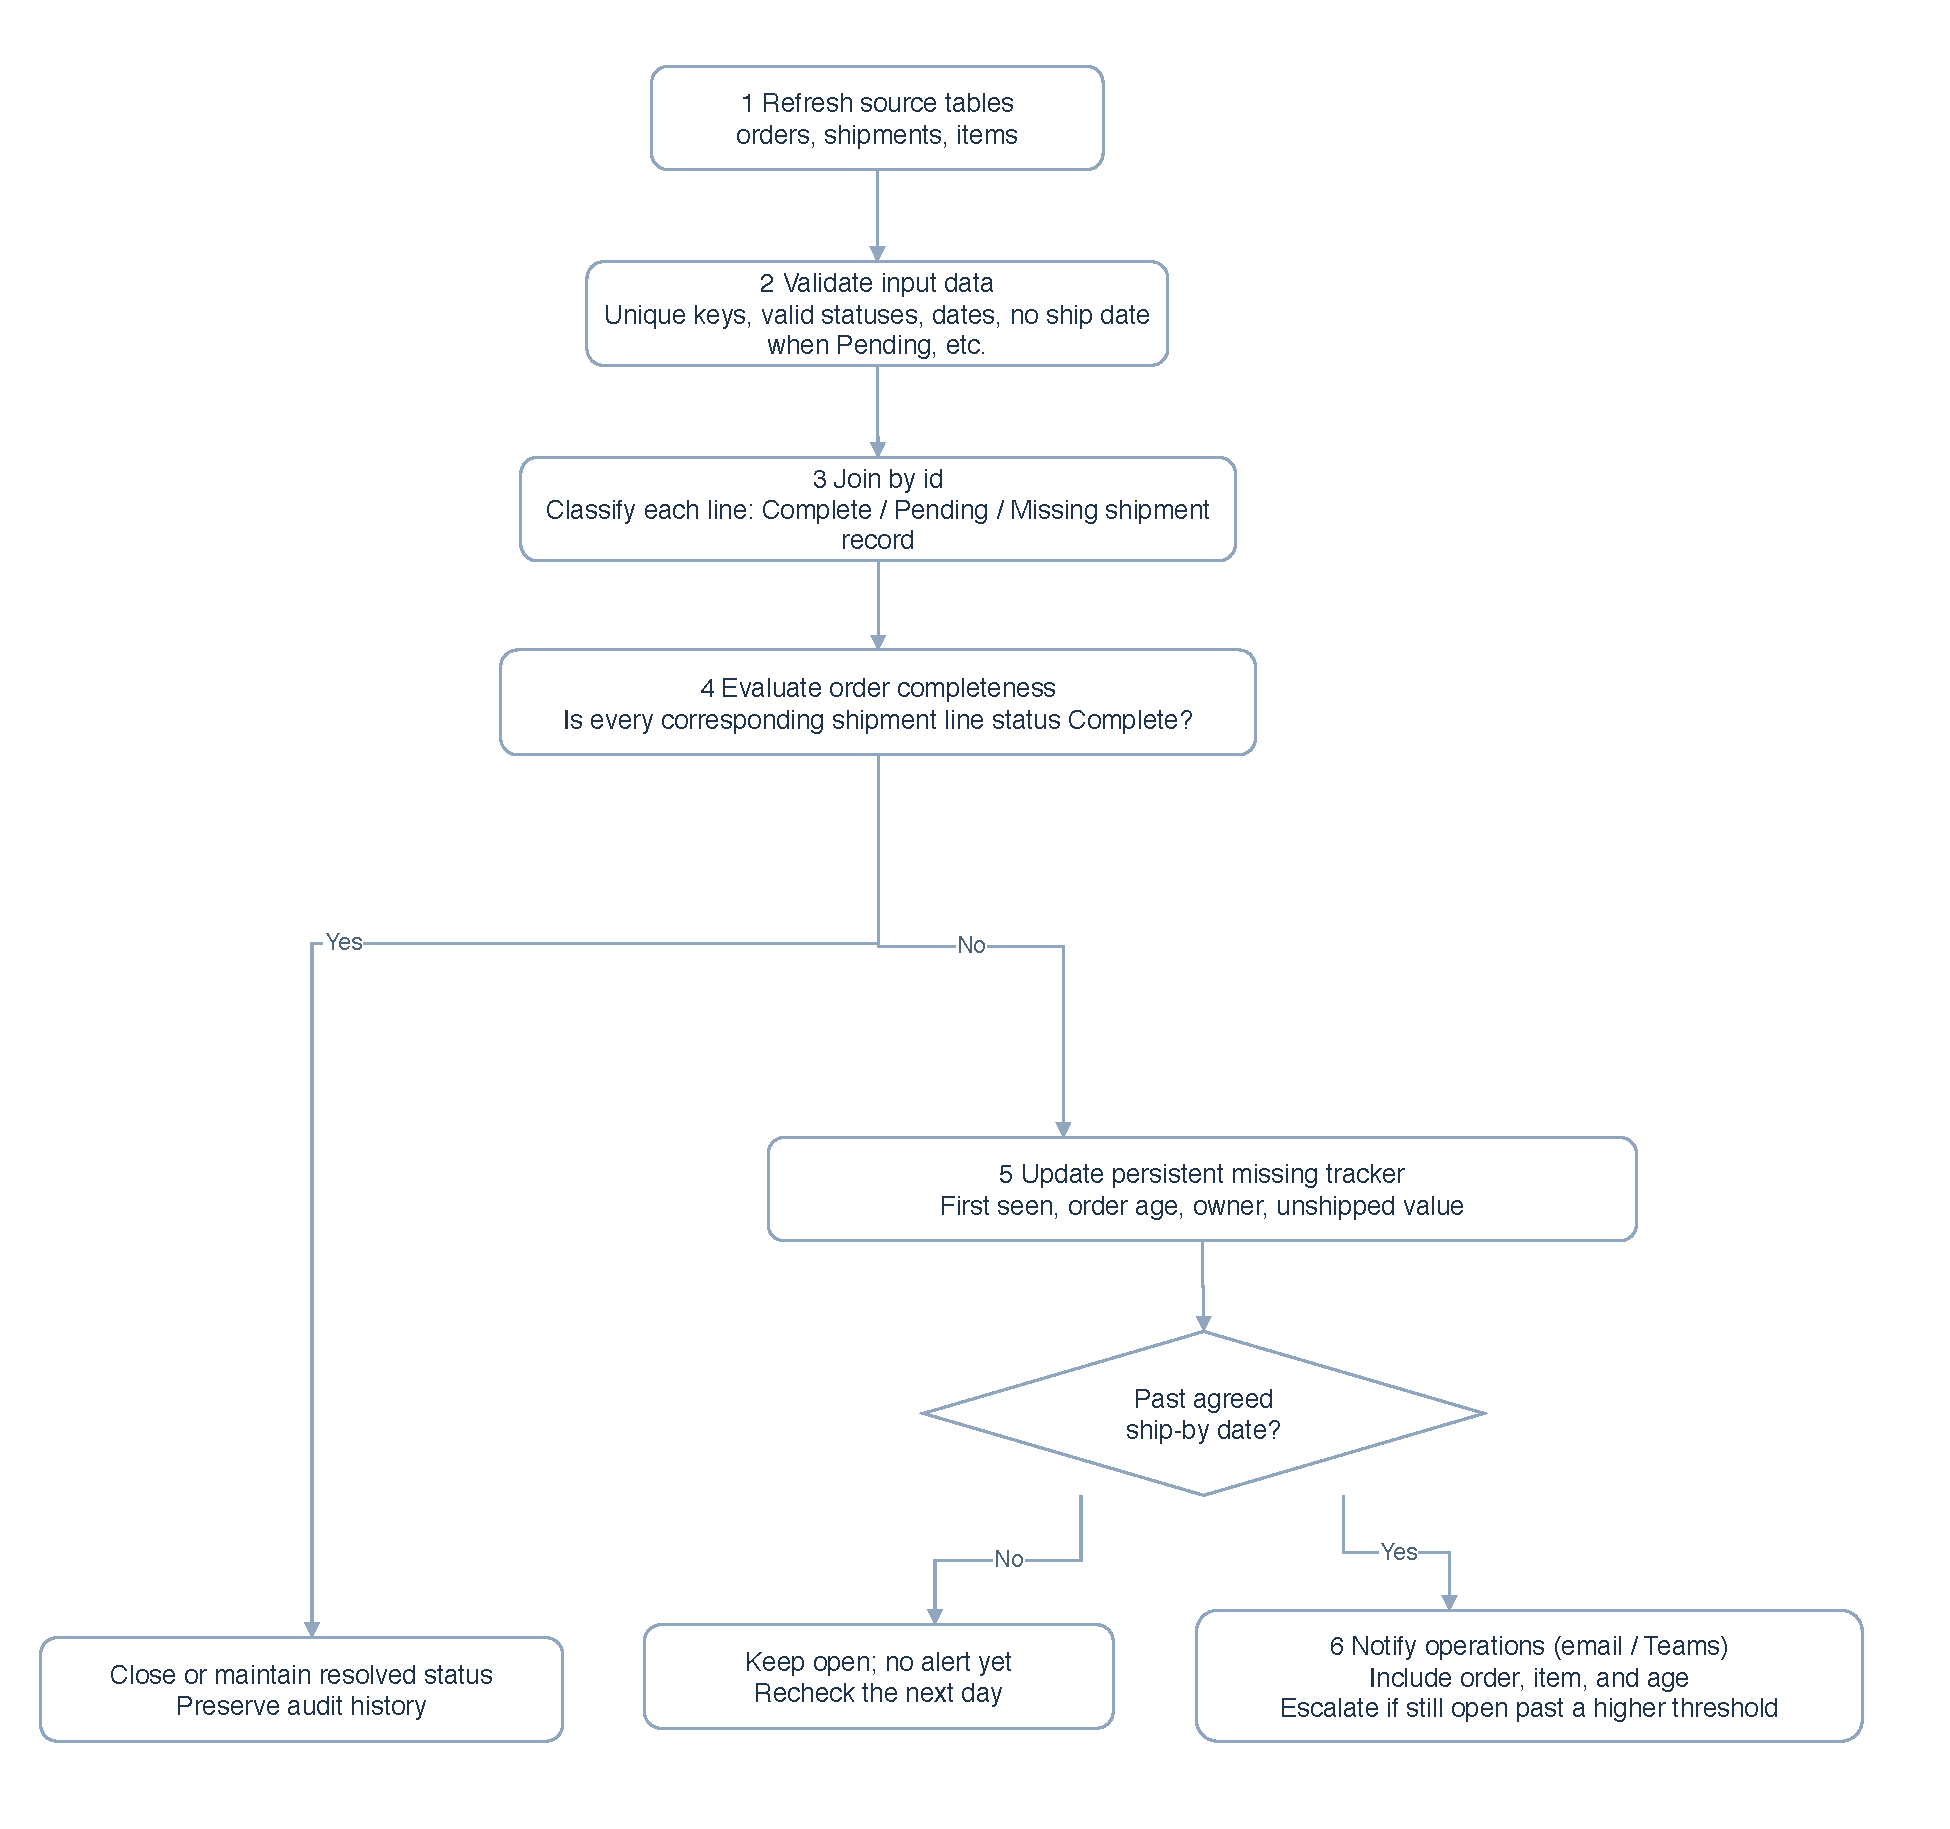
\includegraphics[width=1\linewidth]{diagram.drawio} 

}

\caption{Workflow Visualized}\label{fig:diagram}
\end{figure}

\end{document}
